\documentclass[11pt]{article}
\usepackage{graphicx}
\graphicspath{ {./images/} }
\renewcommand{\figurename}{Fig.}
\begin{document}
\title{Aplicaci\'on de algoritmo gen\'etico: N-queens }
\author{Orlando Hernandez Nu\~nez. Juan Alejandro Bernal Gallego}
\date{21 de Octubre del 2019}
\maketitle

\section{Introducci\'on}
En el presente trabajo se busca dar soluci\'on al problema de las N-queens mediante el uso de un algoritmo gen\'etico. A continuaci\'on, se mostrar\'a la configuraci\'on de par\'ametros con las que fue ejecutado el algoritmo gen\'etico y los resultados obtenidos.

\section{Problema}
En el juego de ajedrez la reina amenaza a aquellas piezas que se encuentren en su misma fila, columna o diagonal. El problema de las 8 reinas (o n-queens ya que dependen del numero asignado) consiste en poner sobre un tablero de ajedrez ocho reinas sin que estas se amenacen entre ellas.
\begin{figure}[h]
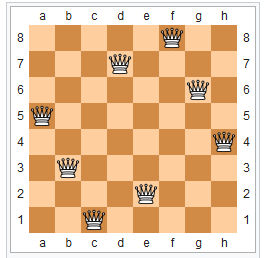
\includegraphics[width=8cm, height=6cm]{nqueens}
\centering
\caption{Soluci\'on al problema de las N-queens}
\end{figure}
\section{Algoritmo Gen\'etico}
\subsection{Definici\'on de la codificaci\'on}
Para representar cada uno de los cromosomas que integrar\'an la poblaci\'on de posibles soluciones
al problema se eligi\'o un vector de n\'umeros enteros donde cada \'indice indica una fila del tablero.
El valor de cada \'indice esta entre 0 y N-1 donde N es el n\'umero de reinas a distribuir en el tablero
y este valor indicar\'a en que columna se ubica la reina dentro del tablero.

Los cromosomas fueron codificados de manera que pudieran representar la ubicaci\'on en columnas y filas de cada reina. El gen representa la columna en la que se encuentra cada reina, y el \'indice del gen representa la posici\'on de las reinas con respecto a las filas.
\begin{itemize}
\item Ejemplo cromosoma \{1, 2, 0, 3\}
\begin{center}
\begin{tabular}{ c c c c }
	0 & 0 & 0 & 1\\
	1 & 0 & 0 & 0\\
	0 & 0 & 1 & 0\\
	0 & 1 & 0 & 0
\end{tabular}
\end{center}
\end{itemize}
\subsection{Funci\'on de fitness}
La funci\'on de fitness se encarga de contar el n\'umero de
cruces en diagonales o en columnas.
\subsubsection{Calcular cruces en diagonales}
Se tiene una posible soluci\'on V y se establece que dos reinas en el tablero estan en la misma diagonal si y solo si:
\[Para\;i \in \{0, 1, 2, ... N-1\}\;y\;j \in \{0, 1, 2, ... N-1\}\;y\;i \neq j;\]
\[V[i] - i == V[j] - j\]
\[V[i] + i == V[j] + j\]
\subsubsection{Calcular cruces en columnas}
Se tiene una posible soluci\'on V de modo que para calcular si dos reinas estan en la
misma columna se cuentan la cantidad de n\'umeros repetidos que hayan dentro de V.
Por ejemplo: Si tenemos [2, 3, 2, 7, 1, 6, 3, 7] se tiene que hay 4 cruces en columna.

Una vez calculadas estas dos cantidades se define la funci\'on de fitness de la siguiente
forma:
\begin{equation}\label{eqfitness}
    fitness = \frac{1}{1+nc}
\end{equation}
Donde nc es el numero de cruces definido como la suma de la cantidad de cruces en diagonal
y los cruces en columnas.
Con la funci\'on de fitness definida de esta forma el objetivo ser\'a
minimizar el n\'umero de cruces de modo que (\ref{eqfitness}) se maximice.

\subsection{Configuraci\'on de par\'ametros}
Los par\'ametros elegidos para la ejecuci\'on del algoritmo gen\'etico se presentan a continuaci\'on:
\begin{equation}
Pcruce = 0.9
\end{equation}
\begin{equation}
Pmutacion = 0.001
\end{equation}
\begin{equation}
Tamano\;de\;poblacion = 20\;individuos
\end{equation}

\section{Resultados}
A continuaci\'on, se presentan los resultados conseguidos con la configuraci\'on
descrita previamente para el algoritmo gen\'etico.
\subsection{Elitista}
Se ejecut\'o el algoritmo hasta alcanzar la iteraci\'on i = 1000  conservando en cada una de las siguientes
generaciones el mejor individuo de la anterior.
la soluci\'on obtenida fue [3, 7, 0, 4, 6, 1, 5, 2]
\begin{center}
\begin{tabular}{ c c c c c c c c }
	0 & 0 & 1 & 0 & 0 & 0 & 0 & 0\\
	0 & 0 & 0 & 0 & 0 & 1 & 0 & 0\\
	0 & 1 & 0 & 0 & 0 & 0 & 0 & 0\\
	0 & 0 & 0 & 0 & 0 & 0 & 1 & 0\\
	0 & 0 & 0 & 0 & 1 & 0 & 0 & 0\\
	1 & 0 & 0 & 0 & 0 & 0 & 0 & 0\\
	0 & 0 & 0 & 0 & 0 & 0 & 0 & 1\\
	0 & 0 & 0 & 1 & 0 & 0 & 0 & 0
\end{tabular}
\end{center}
podemos observar en la figura (\ref{elitismo}) hay 3 curvas, el eje X son el numero de iteraciones y el eje Y representa el valor del fitness. En las 2 curvas online y best-so-far utilizando elitismo destaca un cambio repentino en el promedio de fitness de los individuos y los mejores fitness respectivamente alrededor de la iteraci\'on 300 y 400, mientras que la curva offline no presenta cambios tan grandes durante el proceso evolutivo.
\begin{figure}[t]
    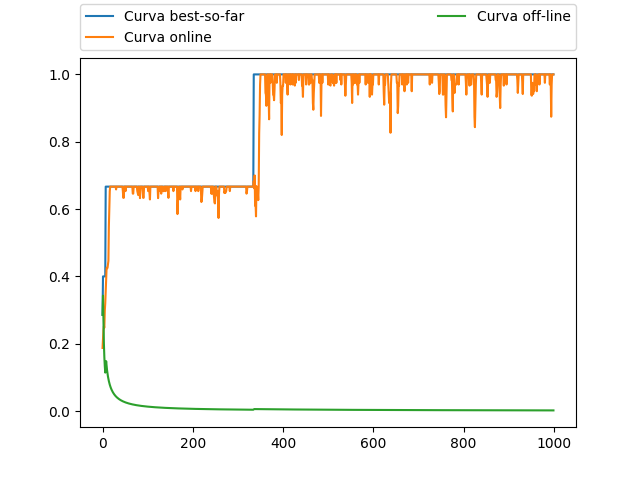
\includegraphics[width=10cm, height=10cm]{Figure_1}
    \centering
    \caption{Curvas de monitoreo ejecuci\'on con elitismo}
    \label{elitismo}
    \end{figure}
\subsection{Sin elitismo}
Se ejecut\'o el algoritmo hasta alcanzar la iteraci\'on i = 1500 sin aplicar elitismo la soluci\'on obtenida fue [5, 2, 0, 7, 4, 1, 3, 6]

\begin{center}
\begin{tabular}{ c c c c c c c c }
	0 & 0 & 0 & 0 & 0 & 0 & 1 & 0\\
	0 & 0 & 0 & 1 & 0 & 0 & 0 & 0\\
	0 & 1 & 0 & 0 & 0 & 0 & 0 & 0\\
	0 & 0 & 0 & 0 & 1 & 0 & 0 & 0\\
	0 & 0 & 0 & 0 & 0 & 0 & 0 & 1\\
	1 & 0 & 0 & 0 & 0 & 0 & 0 & 0\\
	0 & 0 & 1 & 0 & 0 & 0 & 0 & 0\\
	0 & 0 & 0 & 0 & 0 & 1 & 0 & 0
\end{tabular}
\end{center}
En el caso de la figura (\ref{sinelitismo}) se observa que la curva online y best-so-far fluct\'uan menos en el transcurso de las generaciones, y la curva offline tiene una forma similar al de la figura (\ref{elitismo}), encontramos que sin el uso de elitismo se necesita de una mayor cantidad de generaciones para poder encontrar una soluci\'on.
\begin{figure}[h]
    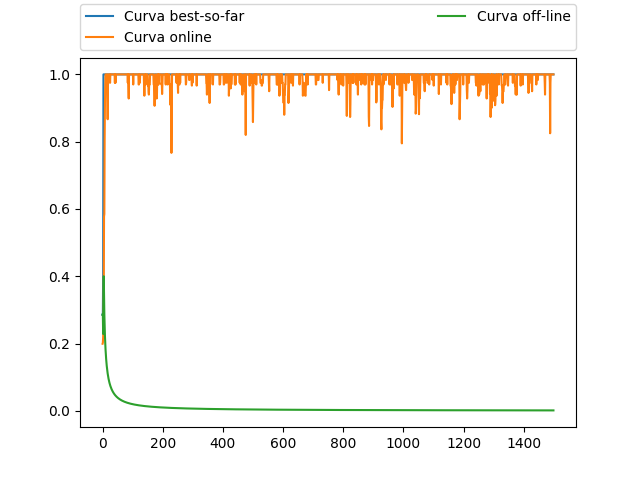
\includegraphics[width=10cm, height=10cm]{Figure_2}
    \centering
    \caption{Curvas de monitoreo ejecuci\'on sin elitismo}
    \label{sinelitismo}
    \end{figure}
\end{document}
